\documentclass[../thesis.tex]{subfiles}
% Separate preamble for this subfile. This preamble is loaded last, so one can override various functions before \begin{document}

% Better comment extension for Vscode colors these comments differently
% Normal comment color
% * Important information
% ! ALERT
% ? Question
% TODO stuff to do
% // This is strikethrough


\begin{document}

\begin{definition}[Lebesgue Space] %? Heil REal analysis book page 269, citation?, page 119+120, chapter 3, Heil metrics and norm
    Let $E$ be a measurable subset of $\R^d$. Given $1 \leq p < \infty$ and a measurable function $f:E\rightarrow \C$, we say that $f$ is \emph{$p$-integrable} if the Lebesgue integral of $|f|^p$ is finite, that is
    \begin{equation*}
        \int_{E} \bralMed{f(t)}^p dt < \infty,
    \end{equation*}
    where $dt= dt_1 \dots dt_d$. We define the \emph{Lebesgue space} $L^p(E)$ as the set of all $p$-integrable functions on $E$, and equip it with the norm
    \begin{equation*}
        \bran{f}_{L^p(E)} = \bracMed{\int_{E} \bralMed{f(t)}^p dt}^{1/p}. \qedhere
    \end{equation*}
\end{definition}

%! %Of all the $L^p$ spaces, the case $p=2$ is special since $L^2(E)$ is the only space whose norm
The case $p=2$ is special since $L^2(E)$ is the only $L^p$ space whose norm is induced by the inner product
\begin{equation*}
    \braaMed{f, g}_{L^2(E)} = \int_{E} f(t)\overline{g(t)} dt,
\end{equation*}
for two functions $f,g\in L^2(E)$. By the Riesz-Fischer theorem \cite[p.~279]{heilIntroductionRealAnalysis2019}, all $L^p$ spaces are complete with respect to the \LPnorm. Hence, $L^2(E)$ is a Hilbert space. 


%* —————————————————————————————————————— C Cont. FUNCTIONS ——————————————————————————————————————
Let
\begin{equation*}  %? Page 102, chapter 3, Heil metrics norms
    C([a,b]) = \braq{f:[a,b] \rightarrow \mathbb{C}: f \text{ is continuous on } [a,b]}
\end{equation*}
denote the set of all continuous, scalar-valued functions whose domain is the closed and bounded interval $\bras{a,b}$. The following useful result with proof can be found in \cite[p.~326]{rudinPrinciplesMathematicalAnalysis20}. 
\begin{lemma}\label{lem:c_dense_L2}
    The set of all continuous functions $C([a,b])$ is dense in the space $L^2([a,b])$ with respect to the \Ltwonorm.
\end{lemma}

%* —————————————————————————————————————— C PERIODIC FUNCTIONS ——————————————————————————————————————
Similarly, let 
\begin{equation*}  %? Page 178, chapter 4, Heil metrics norms
    \Cper([a,b])= \braqMed{f \in C[a,b]: f(a)=f(b)}
\end{equation*}
denote the set of all continuous, real-valued functions on the interval $\bras{a,b}$ satisfying $f(a)=f(b)$. It is periodic in the sense that each element $f$ can be extended to the whole real line by setting 
\begin{equation*}
    f(t+Pn) = f(t), \quad t\in \bras{a,b},
\end{equation*}
for $n\in \Z$ and $P=b-a$. We say that the extended function $f$ is $P$\emph{-periodic}, meaning
\begin{equation*}
    f(t+P) = f(t), \quad t\in \R.
\end{equation*}
%The converse is also true, meaning we have a one-to-one correspondence between elements of $\Cper([a,b])$ and functions that are $P$-periodic on the real line. % if $f'$ is a $P$-periodic function on $\R$, then when $f'$ is restricted to the domain $\bras{a,b}$ it is also an element of $\Cper([a,b])$.
We have a \namecref{lem:c_per_dense_c_and_dense_L2} for $\Cper([a,b])$ similar to \cref{lem:c_dense_L2}, and note that the proof closely follows the one by Heil in \cite[p.~228]{heilMetricsNormsInner2018}.  % although it is never explicitly stated.
\begin{lemma}\label{lem:c_per_dense_c_and_dense_L2}
    The set of all periodic functions $\Cper([a,b])$ is dense in the space $L^2([a,b])$ with respect to the \Ltwonorm.
\end{lemma}
%* The proof of \cref{lem:c_per_dense_c_and_dense_L2} closely follows the proof by Heil in \cite[p.~228]{heilMetricsNormsInner2018} although it is never explicitly stated. 
%Although not stated as explicitly as a result, the proof of \cref{lem:c_per_dense_c_and_dense_L2} can be found in \cite[p.~228]{heilMetricsNormsInner2018}.
\begin{proof}
    \begin{figure}
        \centering
        %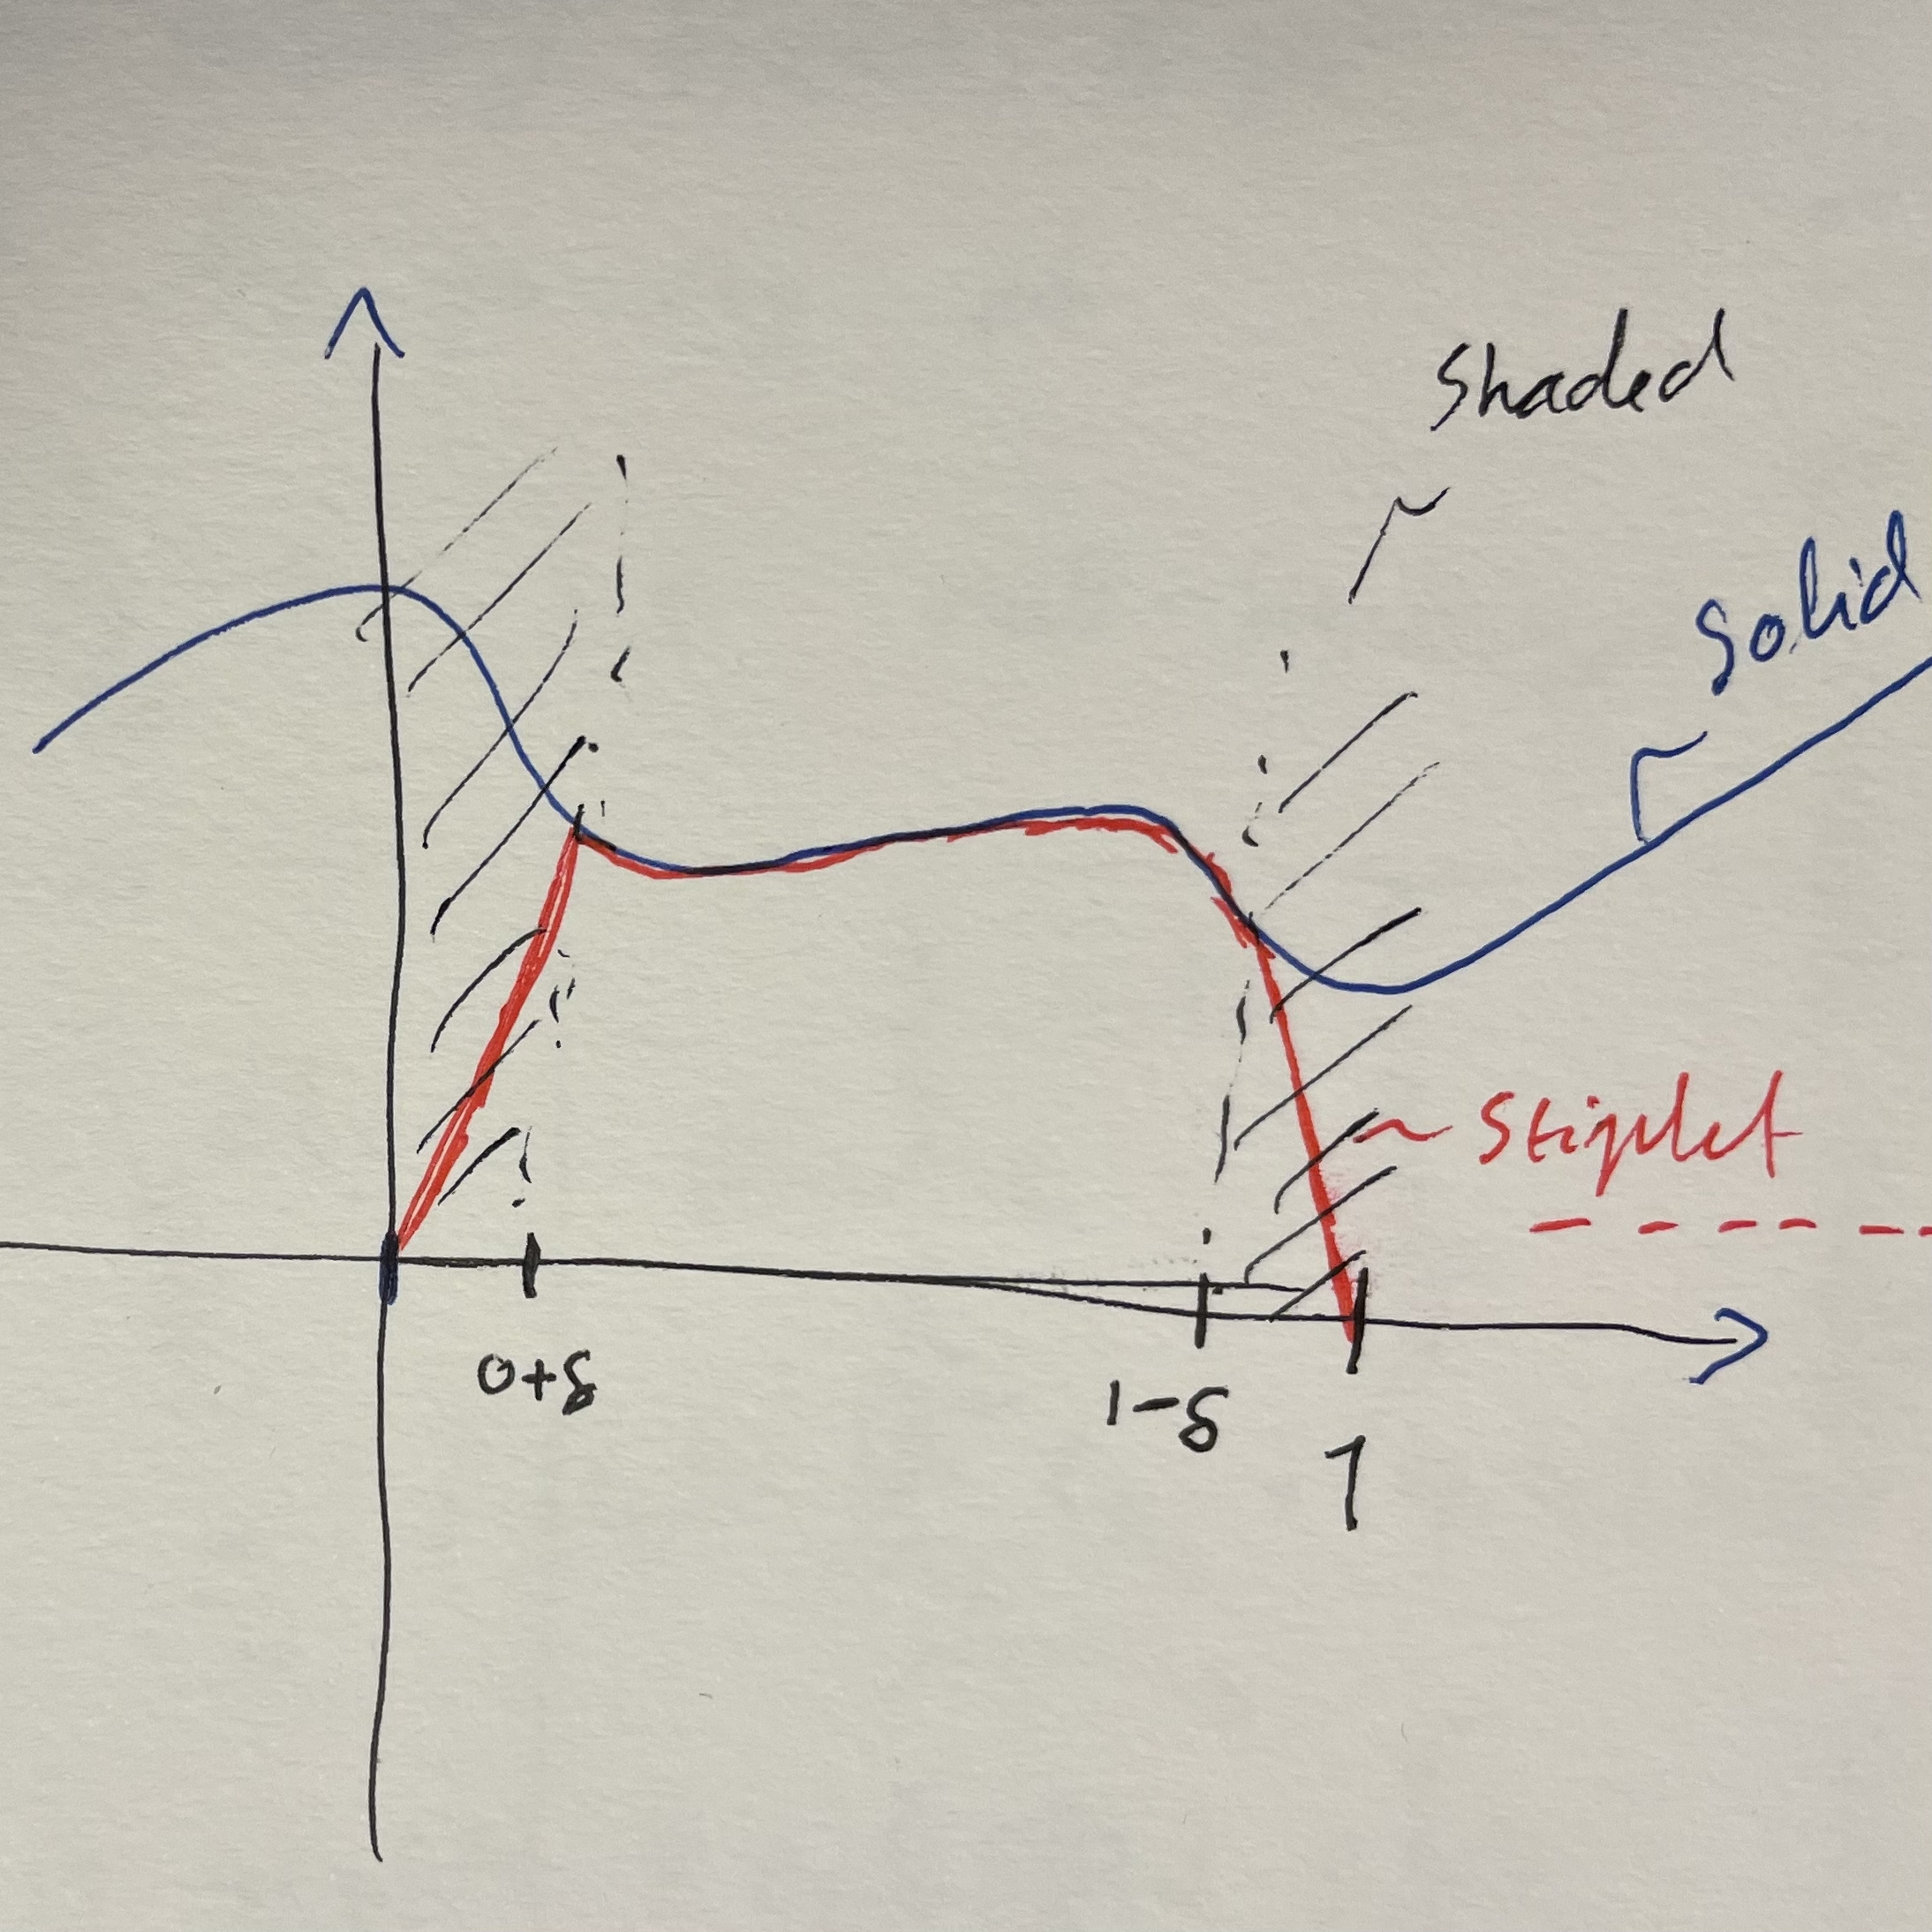
\includegraphics[width=0.45\textwidth]{cper_dense_c.png}
        \input{figures/figure-tex/cper_dense_c.tex}
        \caption{The approximation of the continuous function $f(t)$ in a solid blue by a periodic function $g(t)$ in dashed orange.}
        \label{fig:g_periodic_close_to_f}
    \end{figure}
    %Since $C([a,b])$ is dense in $L^2([a,b])$ from \cref{lem:c_dense_L2}, it will then follow that $\Cper([a,b])$ is dense in $L^2([a,b])$ if we can show that $\Cper([a,b])$ is dense in $C([a,b])$.
    %If we can show that $\Cper([a,b])$ is dense in $C([a,b])$, it will follow that $\Cper([a,b])$ is dense in $L^2([a,b])$, since we know from \cref{lem:c_dense_L2} that $C([a,b])$ is dense in $L^2([a,b])$. 
    If we can show that $\Cper([a,b])$ is dense in $C([a,b])$, it will follow from \cref{lem:c_dense_L2} that $\Cper([a,b])$ is dense in $L^2([a,b])$, since $C([a,b])$ is dense in $L^2([a,b])$. Let $f \in C([a,b])$, $\varepsilon>0$ and $\delta = \varepsilon^2/(8\bran{f}_\infty)$. We aim to construct a piecewise continuous function $g$ which is identical to $f$ on the interval $[a+\delta,b-\delta ]$ and which attains the value $g = 0$ at the endpoints, making $g\in \Cper([a,b])$. We will see that this will change the \Ltwonorm \space by a negligible amount. %In other words, this allows us to approximate any continuous function as closely as we want by a modified (periodic) version of the original function. 
    We construct $g$ in the following way  %. We will see that this will change the \Ltwonorm \space by a negligible amount and only at the expense of two intervals of length $\delta$
    \begin{equation*} % kan lage formel for g på ax+b formel: dvs $dy/dx \cdot x + b$ ELLER  $ -g(b-\delta) / \delta \cdot x + g(b-\delta)/ \delta $ <- dette er høyre side.
        g(t) = 
        \begin{cases} a, &  t=a,\\  
            \text{linear}, &  0<t<a+\delta,\\ 
            f(t), & a+\delta \leq t \leq b-\delta,\\ 
            \text{linear}, &  b-\delta <t<b,\\ 
            a, &  t=b,
        \end{cases}
    \end{equation*} 
    as illustrated in \cref{fig:g_periodic_close_to_f}. Observe that for all $t$ on the interval $[a+\delta, b-\delta]$ we have $\bral{f(t)-g(t)}= 0$, and for all other values of $t$ we know that
    \begin{equation*}
        \bralMed{g(t)} \leq \branMed{g}_{\infty} = \sup_{t\in[a,b]} \bralMed{g(t)} = \sup_{t\in[a+\delta, b-\delta]} \bralMed{g(t)} = \sup_{t\in[a+\delta, b-\delta]} \bralMed{f(t)} \leq \sup_{t\in[a, b]} \bralMed{f(t)} =\branMed{f}_{\infty}
    \end{equation*}
    with equality in the third step using the fact that $g$ is linear and goes towards zero as it approaches $0$ or $b$, and therefore attains its greatest value on the interval $[a+\delta,b-\delta]$ where it is equal to $f$. Using this and the triangle inequality, we have that
    \begin{equation*}
        \bralMed{f(t)-g(t)} \leq \bralMed{f(t)} + \bralMed{-g(t)} \leq \branMed{f}_{\infty} + \branMed{f}_{\infty} = 2 \branMed{f}_{\infty}
    \end{equation*}
    for all $t$ on the intervals $[a, a+\delta]$ and $[b-\delta,b]$. Now,
    \begin{align*}
        \branMed{f-g}_{L^2}^2 &=  \int_0^{a+\delta} \bralMed{f(t)-g(t)}^2 dt + \int_{a+\delta}^{b-\delta} \bralMed{f(t)-g(t)}^2 dt +\int_{b-\delta}^{b} \bralMed{f(t)-g(t)}^2 dt\\ 
        &\leq \int_0^{a+\delta} \bracMed{2 \branMed{f}_{\infty}}^2 dt + 0 +\int_{b-\delta}^{b} \bracMed{2 \branMed{f}_{\infty}}^2 dt\\
        &=  4 \delta \branMed{f}_{\infty}^2 + 4 \delta \branMed{f}_{\infty}^2\\ 
        &= \varepsilon^2
    \end{align*}
    This shows that $\Cper([a,b])$ is dense in $C([a,b])$, which finalizes our proof.
\end{proof}


\end{document}